\chapter{Construção}
\label{cha:Construção}

\section{Tecnologias utilizadas}

Para o armazenamento e consulta dos dados, foi utilizado o banco de dados relacional PostgreSQL \cite{site-postgresql}. O PostgreSQL foi escolhido por ser robusto e eficiente, mas fácil e rápido de configurar. 

O sistema foi separado em interface e API (\textit{Application programming interface}, ou interface de programação da aplicação). Houve a possibilidade de criar o sistema utilizando uma tecnologia que integra a interface e a API, como o Django \cite{site-django}, para evitar a criação de dois serviços separados. Mas como a interface precisava ser bem complexa e interativa, a opção de \textit{templating} do Django não ia ser suficiente. Por isso, a interface foi desenvolvida em Svelte \cite{site-svelte}, um framework em JavaScript \cite{site-js} baseado em componentes, e a API foi desenvolvida com Gin \cite{site-gin}, um framework em Go. \cite{site-go}. A lógica do algoritmo foi implementada dentro do serviço da API.

A coleta dos dados provenientes do Microhorario e a autenticação com o sistema acadêmico universitário foi desenvolvida em serviços menores, cada um com uma única funcionalidade, separados da API (microserviços). Ambos foram desenvolvidos utilizando o framework Flask \cite{site-flask}, utilizando a linguagem \cite{site-python}.

A figura \ref{fig:diagrama-arquitetura} exibe um diagrama da arquitetura do sistema.
% Cada um dos componentes serão explicados nas próximas secções do capítulo.

\begin{figure}[ht]
    \begin{center}
    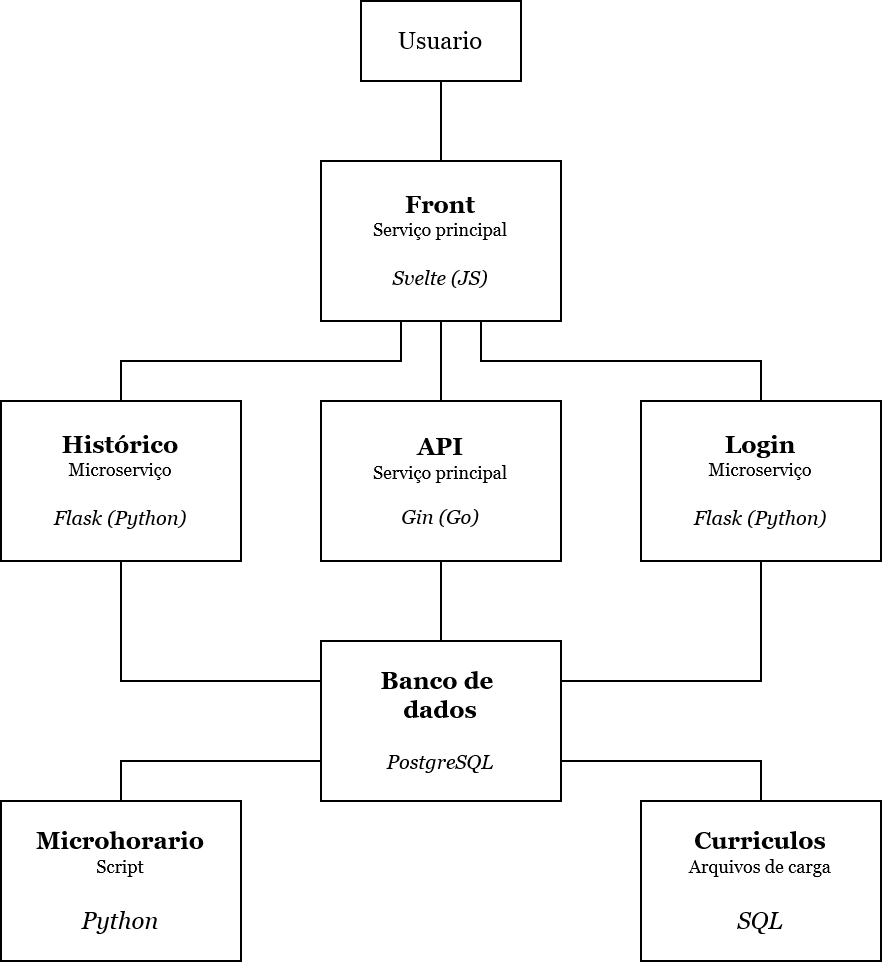
\includegraphics[width=300pt]{figuras/diagrama-arquitetura.png}
    \caption{Diagrama da arquitetura do sistema}
    \label{fig:diagrama-arquitetura}
    \end{center}
\end{figure}

\section{Coleta de dados}

O o modelo lógico representado na figura \ref{fig:modelo-logico} define a construção de catorze tabelas no banco de dados. O trecho de código \ref{cod:sql-create} contém o modelo físico do banco de dados, ou seja o código SQL que define a modelagem das tabelas.

\lstinputlisting[label=cod:sql-create,title={create.sql},caption={Modelo físico},language=SQL]{codigo/10-create.sql}

Além dos dados gerados pela interação do usuário, o sistema precisa de dados provenientes da faculdade, como as disciplinas, turmas, professores e currículos. Esses dados são coletados ocasionalmente, exceto os currículos, que foram coletados e inseridos somente uma vez.

Como o algoritmo e o sistema foi planejado para o departamento de informática, a quantidade de currículos a ser inserida é pequena. No total, foram inseridos seis currículos: três de engenharia de computação (Currículos 2023, 2018.0 e 2018.1) e três de ciência de computação, disponíveis nas respectivas páginas
\footnote{\url{https://www.puc-rio.br/ensinopesq/ccg/eng_computacao.html}}
\footnote{\url{https://www.puc-rio.br/ensinopesq/ccg/ciencia_computacao.html}}
dos cursos.

Os dados do currículo foram transformados manualmente em um arquivo no formato SQL, executado ao criar o banco de dados. O trecho de código \ref{cod:sql-curriculo} contém um exemplo de um dos seis arquivos criados, um para cada currículo.

\lstinputlisting[label=cod:sql-curriculo,title={curriculo-cie-18-0.sql},caption={Exemplo do arquivo de carga de currículos},language=SQL]{codigo/10-curriculos.sql}

Os dados provenientes das disciplinas e turmas são coletados diretamente através do microhorário. Existe uma biblioteca  
\footnote{Dispon\'ivel em: \url{https://pypi.org/project/microhorario-dl/}}
Python que permite baixar todos as informações disponíveis no microhorário, e opcionalmente coletar as ementas e pré-requisitos que estão disponíveis em página. A biblioteca baixa os dados das disciplinas e turmas em menos de três segundos, mas para também baixar as ementas e pré-requisitos que estão em um outro serviço, a biblioteca demora cerca de 30 minutos. Portanto, foi criado um módulo, chamado \verb|microhorario|, que permite atualizar o banco com as informações básicas das disciplinas e turmas, mas que pode ser alterado para atualizar também as ementas e pré-requisitos. Esse módulo foi configurado de forma a ser executado na sua forma mais simples uma vez a cada hora, e executado na forma completa uma vez por semana.

\section{Definição e implementação do algoritmo}

O algoritmo busca satisfazer as necessidades apresentadas na tabela \ref{tab:entrevista-criterios-peso}. As entrevistas indicaram a importância de cinco categorias (Conteúdo, Professor, Avaliação, Horário e Opinião). Por isso, o algoritmo foi dividido nessas cinco categorias.

O algoritmo se baseia num valor $V[d,u]$ atribuído a cada disciplina, que indica a relevância da disciplina $d$ para o usuário $u$. O valor $V[d,u] \in [0, 1]$,
sendo 1 o maior grau de relevância da disciplina, e 0 o menor. O cálculo de $V$ é uma média ponderada, conforme a equação \ref{equ:algoritmo-valor}

\begin{equation}
\label{equ:algoritmo-valor}
    V[d,u] = P_cV_c[d,u] + P_pV_p[d,u] + P_aV_a[d,u] + P_hV_h[d,u] + P_oV_o[d,u]
\end{equation}

Onde $d$ é uma disciplina, $u$ é um usuário, $P_x[d,u]$ é o valor de uma das cinco categorias para a disciplina $d$ e o usuário $u$, e $P_x$ é o peso de uma das cinco categorias.

O valor $V_c[d,u]$ indica o quão relevante é a disciplina para o aluno de acordo com o seu conteúdo. Para isso, o valor é calculado de acordo com o histórico de outros alunos e com o currículo do aluno, conforme a equação \ref{equ:algoritmo-conteudo}:

\begin{equation}
\label{equ:algoritmo-conteudo}
    V_c[d,u] = 
    \begin{dcases}
        1.0                                                        ,\: d \in Historico[u] \\ 
        \frac{|\, A_{cursou}[d,u] \,|}{|\,  A_{curriculo}[u] \,|}   ,\: \text{caso contrário}
    \end{dcases}
\end{equation}

Em que $A_{cursou}[d,u]$ representa o conjunto de alunos do mesmo currículo que o usuário $u$ que cursaram a disciplina $d$, e $A_{curriculo}[u]$ representa o conjunto de todos os alunos do mesmo currículo do usuário $u$. Em resumo, o valor $V_c[d,u]$ é o valor máximo caso a disciplina deve ser cursada pelo usuário, ou sendo uma eletiva é a proporção de alunos do mesmo currículo que fizeram esta disciplina. Essa proporção indica se o conteúdo é relevante para alunos semelhantes ao usuário.

%% TODO: outras categorias

\section{Implementação da API}

\section{Implementação da interface}